\documentclass[10pt, reqno]{amsart}
\usepackage[margin = 0.5 in]{geometry}
\usepackage{multicol}
\usepackage{float}
\usepackage{fancyhdr}
\usepackage{graphicx}
\usepackage{hyperref}
\usepackage{fancyvrb}

\setlength{\abovecaptionskip}{5pt plus 3pt minus 3pt}

\hypersetup{colorlinks=true,allcolors=blue}
\pagestyle{fancy} \fancyhead{} \fancyfoot[C]{\normalsize\thepage}
\renewcommand{\headrulewidth}{0pt}
\begin{document}
\title{CFDG Undergraduate Research Summary \quad Jacob Ivanov}

\maketitle

\begin{multicols}{2}
\vspace{-.1 in}
\section{Summary}
As an Undergraduate Research Assistant in the Computational Fluid Dynamics Group under Dr. Georgios Matheou, one of my main contributions was the development of a spectral interpolation algorithm for 1-3 spatial dimensions, that is portable to any common scientific computing language. Tested versions in Python and MATLAB were completed, as well as proofs of concept in C and Julia. 

Additionally, I implemented a numerical solution of Perturbed Taylor-Green Turbulence using the Vorticity-Streamfunction method, where I am currently implementing particle tracking. Dr. Matheou was helpful in giving advice and direction, but all implementations were solely my work. 
\vspace{-.05 in}
\section{Spectral Interpolation Algorithm}
It is often advantageous to perform operations in frequency space rather than physical space. By using a spectral interpolation algorithm on the frequency-space variables, we can obtain physical-space values at intermediate positions.
\vspace{-.1 in}
\begin{figure}[H]
    \centering
    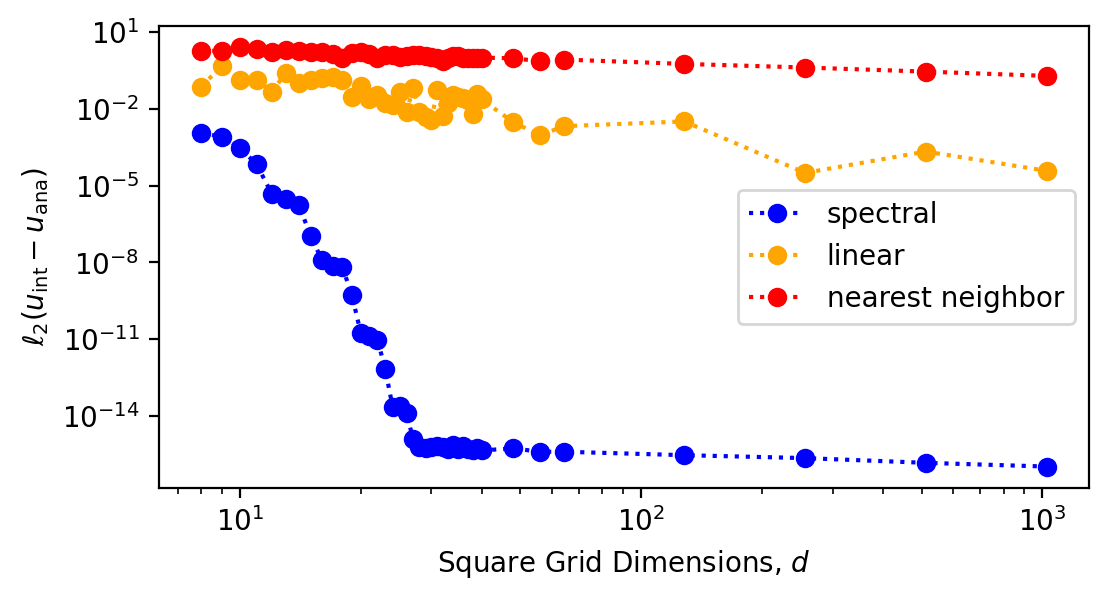
\includegraphics[width=1\linewidth]{Comparison of Interpolation Convergence by Method.png}
    \caption{Comparison of Interpolation Error Convergence by Method}
    \label{fig:1}
\end{figure}
\vspace{-.1 in}
This method's accuracy was shown to converge to within an order of machine epsilon for smooth functions on a discrete grid larger than roughly $30 \times 30$, much more rapidly than nearest-neighbor or linear interpolation methods, which can be seen in Fig.~\ref{fig:1}, which was tested on the function $u(x, y) = \exp \Bigl[ \sin(x) \cos(y) \Bigr]$, which is representative of any smooth periodic function without a finite Fourier series.
\vspace{-.05 in}
\section{Perturbed Taylor-Green Turbulence}
In order to test this algorithm in a real application, a 2D turbulence model was developed with the Spectral Voriticity-Streamfunction Method. The equation for incompressible (i.e. $\nabla \cdot \vec{u} \equiv 0$) vorticity evolution is as follows:
\begin{equation}\label{eqn:1}
    \partial_t \left[ \omega \right] = \nu \left( \partial_x^2 + \partial_y^2 \right) \left[ \omega \right] - \Big( u \cdot \partial_x \left[ \omega \right] + v \cdot \partial_y \left[ \omega \right] \Big)  
\end{equation}
By using discrete spectral methods, where we assume periodicity and smoothness, we obtain the following:
\begin{equation}\label{eqn:2}
    \begin{aligned}
    \partial_t \left[ \Omega_{pq} \right] = & - \nu \left( k_p^2 + k_q^2 \right) \left[ \Omega_{pq} \right] \\
    & - \mathrm{fft2} \Big( u_{ij} \cdot \partial_x \left[ \omega_{ij} \right] + v_{ij} \cdot \partial_y \left[ \omega_{ij} \right] \Big) 
    \end{aligned}
\end{equation}
This equation is transformed with an integrating factor to be:
\begin{equation}\label{eqn:3}
    \Xi_{pq} = \exp \left[ \nu \left(k_p^2 + k_q^2 \right) t \right]
\end{equation}
\begin{equation}\label{eqn:4}
    \partial_t \Big[ \Xi_{pq} \Omega_{pq} \Big] = - \underline{i} \Xi_{pq} \Big[ k_p \cdot \mathrm{fft2}(u_{ij} \omega_{ij}) + k_q \cdot \mathrm{fft2}(v_{ij} \omega_{ij}) \Big]
\end{equation}
Equation~\eqref{eqn:4} was then numerically integrated using a 3rd-order Runge-Kutta method. $\Omega_{pq} = \mathrm{fft2} \Big[ \nabla \times \vec{u}_{ij} \Big]$ was initialized with the following:
\begin{equation}\label{eqn:5}
    u_{ij} = +\cos(\beta x_i) \cdot \sin(\beta y_j) + \gamma_u 
\end{equation}
\begin{equation}\label{eqn:6}
    v_{ij} = -\sin(\beta x_i) \cdot \cos(\beta y_j) + \gamma_v 
\end{equation}
where $\gamma_u$ and $\gamma_v$ represent \verb|rng|-generated perturbations to $u$ and $v$, respectively. Turbulence was then sustained by modifying the $\Xi_{pq}$ variable to be negative for a thin range of higher wavenumbers and boosted for very low wavenumbers. The resultant turbulence can be seen in Fig.~\ref{fig:2}.
\vspace{-.1 in}
\begin{figure}[H]
    \centering
    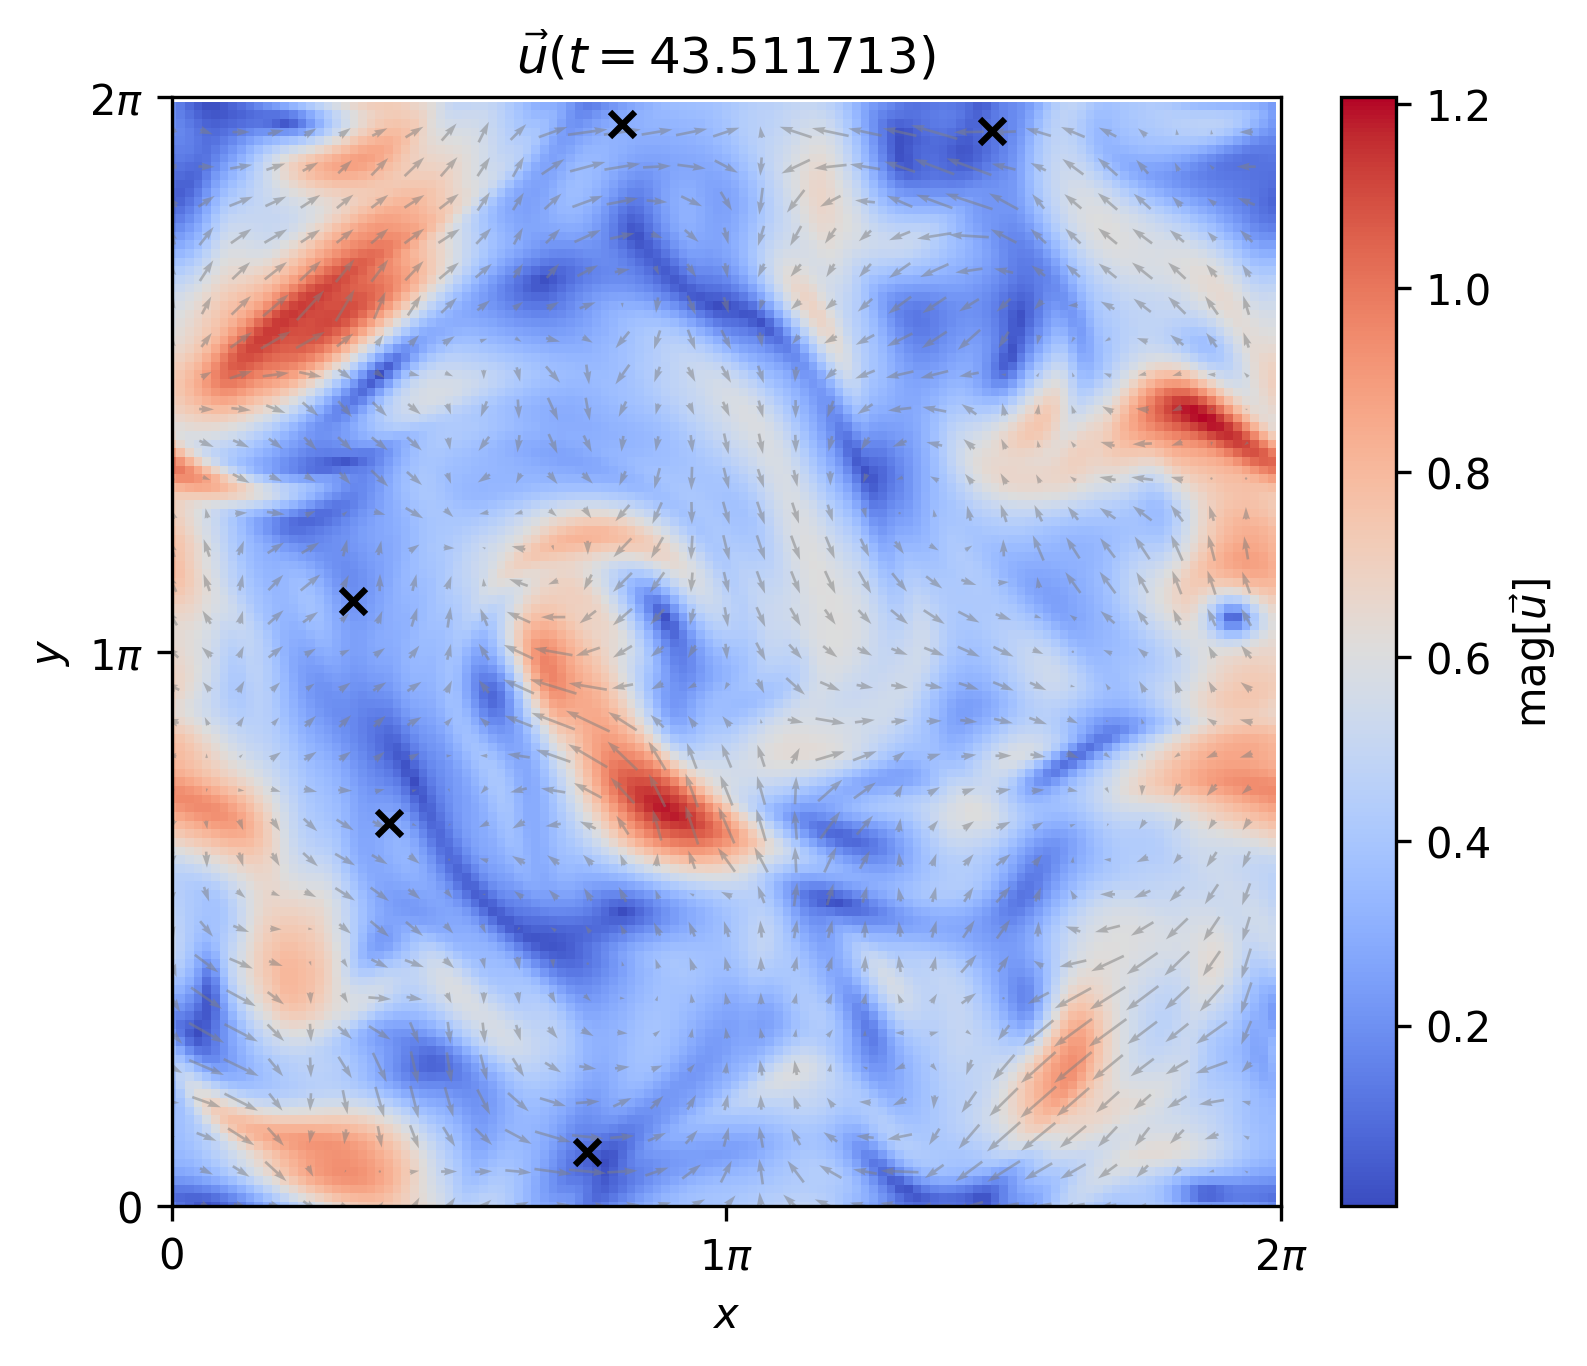
\includegraphics[width=1\linewidth]{velocity field t = 43.51171.png}
    \caption{Perturbed Taylor-Greene Turbulence with Particle Tracking}
    \label{fig:2}
\end{figure}
\vspace{-.1 in}
Particle tracking was implemented with a simple Euler integration of the spectrally interpolated velocities at the particle point, and a Predictor-Corrector method is currently in development. 
\vspace{-.15 in}
\section{Conclusion}
In conclusion, through my research with Dr. Matheou, which I believe to be the best example of my work, I was able to develop a broad understanding of numerical and computational methods as they apply to fluid dynamics. 
I believe the skills that I have developed have prepared me for graduate-level research in the fields of super/hypersonic propulsion. 
\end{multicols}

\end{document}